\documentclass[11pt,a4paper]{article}

% --- Packages ---
\usepackage[utf8]{inputenc}
\usepackage[italian]{babel}
\usepackage[T1]{fontenc}
\usepackage{lmodern}
\usepackage{geometry}
\geometry{left=1.8cm, right=1.8cm, top=1.8cm, bottom=1.8cm}
\usepackage{enumitem}
\usepackage{titlesec}
\usepackage{hyperref}
\usepackage{xcolor}
\usepackage{tabularx}
\usepackage{graphicx}

% --- Color Definitions ---
\definecolor{color0}{rgb}{0,0,0}         % Main text color (Black)
\definecolor{color1}{RGB}{0, 75, 135}    % Academic Blue
\definecolor{color2}{gray}{0.3}          % Secondary info color

% --- Section Styling ---
\titleformat{\section}
  {\Large\bfseries\color{color1}}
  {}{0em}{}
  [\titlerule]
\titlespacing{\section}{0pt}{14pt}{8pt}

% --- Hyperref Setup ---
\hypersetup{
    colorlinks=true,
    linkcolor=color1,
    urlcolor=color1,
    pdftitle={Davide Chirichella - Curriculum Vitae},
}

% --- Custom Entry Commands ---
\newcommand{\cvitem}[2]{
    \noindent
    \begin{tabularx}{\textwidth}{@{}p{3.8cm} X@{}}
        \textbf{#1} & #2
    \end{tabularx}
    \vspace{3pt}
}

\usepackage{etoolbox}
\newcommand{\cventry}[6]{
    \noindent
    \begin{tabularx}{\textwidth}{@{}p{3.8cm} X@{}}
        {\small\sffamily #1} & \textbf{#2} \\
        \ifstrempty{#3}{%
            \ifstrempty{#4}{%
                \ifstrempty{#5}{}{& \small #5 \\}%
            }{& #4\ifstrempty{#5}{}{\\ & \small #5} \\}%
        }{%
            & \textit{#3}\ifstrempty{#4}{}{, #4}\ifstrempty{#5}{}{\\ & \small #5} \\%
        }%
        & \small #6
    \end{tabularx}
    \vspace{10pt}
}

\begin{document}

\pagestyle{empty}

% --- Header ---
\noindent
\begin{minipage}[t]{0.80\textwidth}
    \raggedright
    {\Huge \textbf{Davide Chirichella}} \\
    \vspace{2mm}
    {\large \textcolor{color1}{Studente Magistrale in Ingegneria Informatica | Sistemi Distribuiti \& Junior DevOps Engineer}}
\end{minipage}
\begin{minipage}[t]{0.20\textwidth}
    \raggedleft
    \vspace{-4mm}
    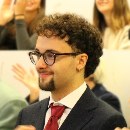
\includegraphics[width=2.1cm]{picture.png}
\end{minipage}

\vspace{4mm}

\section{Informazioni Personali}
\cvitem{Nome e Cognome}{Davide Chirichella}
\cvitem{Data di Nascita}{10 Novembre 2003}
\cvitem{Cittadinanza}{Italiana}
\cvitem{Residenza attuale}{Bologna, Italia}
\cvitem{Email}{\href{mailto:davidechirichella10@gmail.com}{davidechirichella10@gmail.com} | \href{mailto:davide.chirichella@unibo.it}{davide.chirichella@unibo.it}}
\cvitem{LinkedIn}{\href{https://www.linkedin.com/in/davide-chirichella-88200b1ba/}{linkedin.com/in/davide-chirichella-88200b1ba}}
\cvitem{GitHub}{\href{https://github.com/chirichexe}{github.com/chirichexe}}

\section{Profilo}
\noindent Junior engineer e studente magistrale in \textbf{Ingegneria Informatica} presso l'Università di Bologna con esperienza pratica in \textbf{sistemi distribuiti}, \textbf{architetture cloud-native} e \textbf{pratiche DevOps}. Specializzato nel design e nella gestione di sistemi a microservizi scalabili utilizzando Kubernetes e infrastructure-as-code. L'esperienza spazia dallo sviluppo backend all'automazione CI/CD e architetture cloud-edge per ambienti IoT.

\section{Istruzione}
\cventry{2025 -- In corso}{Laurea Magistrale in Ingegneria Informatica}{Alma Mater Studiorum --- Università di Bologna}{Bologna}{Media attuale: 29.5/30}{Focus su Sistemi Distribuiti, Calcolo Parallelo e architetture Cloud-native.}

\cventry{2022 -- 2025}{Laurea Triennale in Ingegneria Informatica}{Alma Mater Studiorum --- Università di Bologna}{Bologna}{Voto: 107/110}{
\begin{itemize}[noitemsep, topsep=0pt, leftmargin=1em]
    \item \textbf{Tesi (Tirocinio curriculare presso il DISI):} ``Analisi delle prestazioni e monitoraggio in ambienti Cloud-Edge per l'Internet of Things''
    \item Sviluppo di un sistema distribuito cloud-edge per l'orchestrazione di dispositivi IoT utilizzando Kubernetes Operator, Crossplane e Istio Service Mesh.
    \item Progettazione di uno stack di osservabilità completo con Prometheus, Grafana e OpenTelemetry.
\end{itemize}}

\cventry{2017 -- 2022}{Diploma di Maturità Scientifica}{Liceo Scientifico Galileo Galilei}{Potenza}{}{Focus su Adobe Creative Cloud, produzione di contenuti multimediali e Graphic Design.}

\section{Esperienza Lavorativa}
\cventry{Feb 2026 -- In corso}{Junior DevOps Engineer}{HoDiritto (Startup)}{Ibrido}{}{
\begin{itemize}[noitemsep, topsep=0pt, leftmargin=1em]
    \item Lead del system design e dell'architettura infrastrutturale per un MVP in fase iniziale.
    \item Gestione della containerizzazione dei servizi e implementazione di best practice per la sicurezza delle API.
    \item Provisioning dell'infrastruttura cloud tramite Terraform e automazione delle pipeline CI/CD.
    \item Configurazione dello stack di osservabilità completo e gestione del setup di DNS, server e sistemi mail aziendali.
\end{itemize}}

\cventry{Feb 2026 -- In corso}{Tutor Didattico (Amministrazione di Sistema)}{Alma Mater Studiorum --- Università di Bologna}{Bologna}{}{
\begin{itemize}[noitemsep, topsep=0pt, leftmargin=1em]
    \item Supporto al corso di laurea triennale ``Amministrazione di Sistema e Sicurezza''.
    \item Guida pratica sull'amministrazione di sistemi Linux, shell scripting e pratiche di sicurezza.
    \item Assistenza agli studenti nel debugging e nella risoluzione di problemi a livello di sistema.
\end{itemize}}

\cventry{2023 -- 2026}{Software Engineer}{Project Quality Systems S.R.L.}{Remoto}{}{
\begin{itemize}[noitemsep, topsep=0pt, leftmargin=1em]
    \item Sviluppo e manutenzione di un'applicazione desktop C\# per la gestione degli audit.
    \item Progettazione e implementazione di funzionalità full-stack utilizzando React.js, Node.js e MySQL.
    \item Contributo all'evoluzione di una piattaforma gestionale aziendale.
    \item Collaborazione nell'analisi dei requisiti e nel design delle funzionalità.
\end{itemize}}

\section{Progetti}
\cventry{}{Piattaforma di orchestrazione IoT Cloud-Edge (Progetto di tirocinio)}{}{}{}{
\begin{itemize}[noitemsep, topsep=0pt, leftmargin=1em]
    \item Progettazione di un'architettura distribuita per la gestione di dispositivi IoT a basso consumo in ambienti edge e cloud tramite Istio e Kubernetes.
    \item Implementazione di Custom Resource e controller Kubernetes per l'orchestrazione dei dispositivi.
    \item Integrazione di Crossplane per il provisioning dinamico dell'infrastruttura.
    \item Sviluppo di una pipeline di osservabilità tramite Prometheus, Grafana e OpenTelemetry.
\end{itemize}}

\cventry{}{Contributi Open-source (GitHub)}{}{}{}{
\begin{itemize}[noitemsep, topsep=0pt, leftmargin=1em]
    \item Contributi a sistemi distribuiti e progetti relativi al mondo DevOps.
    \item Focus su tooling per Kubernetes, automazione e workflow cloud-native.
\end{itemize}}

\section{Competenze Tecniche}
\cvitem{Linguaggi}{Go, C, Java, C\#, JavaScript (React.js, Node.js), Python, SQL, database NoSQL, CUDA.}
\cvitem{Cloud \& DevOps}{Kubernetes, Docker, Terraform, Ansible, Vagrant, pipeline CI/CD, Istio, Crossplane.}
\cvitem{Osservabilità}{Prometheus, Grafana, OpenTelemetry.}
\cvitem{Sistemi \& IoT}{Amministrazione sistemi Linux, shell scripting, MQTT, Cybersecurity.}
\cvitem{Strumenti}{Git, Adobe Creative Suite (Photoshop, Illustrator, Premiere).}

\section{Lingue}
\cvitem{Italiano}{Madrelingua.}
\cvitem{Inglese}{B2 - Cambridge English First (FCE).}

\vfill

\begin{minipage}[t]{0.5\textwidth}
    \raggedright
    \small Bologna, \today
\end{minipage}
\begin{minipage}[t]{0.5\textwidth}
    \raggedleft
    \small \textit{Davide Chirichella} \\[1.2cm]
    \rule{5cm}{0.4pt}
\end{minipage}

\vspace{1.5cm}
\noindent
\begin{minipage}{\textwidth}
    \centering
    \scriptsize
    Autorizzo il trattamento dei miei dati personali presenti nel curriculum vitae ai sensi del Decreto Legislativo 30 giugno 2003, n. 196 e dell’art. 13 del GDPR (Regolamento UE 2016/679) ai fini della ricerca e selezione del personale.
\end{minipage}

\end{document}
